\originalchapter{8.09作业十}
题源: Assignment 10, 2014年12月5日18时截止, 实际题面PDF第2--5页. 以下五题全部采用AI独立解答或独立数值复现, 没有可取得的官方答案. 相图采用确定方程或实际数据, 不把示意形状作为稳定性证明.

\begin{exercise}
原题1（8分）. 求$\dot x=x(4+y-x^2)$、$\dot y=y(x-1)$全部固定点、类型、稳定性与有用的本征方向, 画平面轨迹粗图.
\end{exercise}
\begin{solution}
第二式给$y=0$或$x=1$. 全部固定点为$(0,0),(2,0),(-2,0),(1,-3)$. Jacobian为$J=\bigl(\begin{smallmatrix}4+y-3x^2&x\\y&x-1\end{smallmatrix}\bigr)$. 在原点根为$4,-1$, 分别沿$(1,0),(0,1)$, 是鞍点. 在$(2,0)$根$-8,1$, 向量$(1,0),(2/9,1)$, 是鞍点. 在$(-2,0)$根$-8,-3$, 向量$(1,0),(-2/5,1)$, 是稳定结点. 在$(1,-3)$根$-1\pm i\sqrt2$, 是稳定焦点, 复本征向量可取$(1,1\pm i\sqrt2)$; 在该点右侧小位移$(\varepsilon,0)$有$\dot y=-3\varepsilon$, 所以局部顺时针.

$x=0$和$y=0$都是不变轴, 不能让粗图轨迹穿轴. 其余零流线是$y=x^2-4$和$x=1$. 各区域箭头的符号直接由$x(4+y-x^2)$与$y(x-1)$确定. 下图为实际积分的有限时相轨道及固定点, 不从有限绘图声称全局分类完毕.
\end{solution}
\begin{center}
\begin{tikzpicture}
\begin{axis}[width=.75\textwidth,height=5.5cm,xlabel={$x$},ylabel={$y$},xmin=-3,xmax=3,ymin=-5,ymax=1.5,grid=major]
\foreach \idx in {0,...,7}{\addplot[no marks]table[x=x,y=y,col sep=comma]{figures/fixedpoint-\idx.csv};}
\addplot[only marks,mark=*,mark size=2pt]coordinates{(0,0)(2,0)(-2,0)(1,-3)};
\node[anchor=south west]at(axis cs:0,0){鞍};\node[anchor=south west]at(axis cs:2,0){鞍};
\node[anchor=south east]at(axis cs:-2,0){结点};\node[anchor=south]at(axis cs:.9,-2.2){焦点};
\draw[->,thick](axis cs:1.8,-3.5)--(axis cs:1.45,-3.7);
\draw[->,thick](axis cs:-1,.7)--(axis cs:-1.3,.58);
\draw[->,thick](axis cs:.8,-2.5)--(axis cs:.9,-2.43);
\end{axis}
\end{tikzpicture}
\end{center}


\begin{exercise}
原题2（15分）. 质量$m$的珠沿半径$a$的竖直圆环滑动, 摩擦系数$\beta>0$, 圆环绕竖轴以恒速$\omega_0$转动. 方程为$ma\ddot\theta=-\beta\dot\theta+ma\omega_0^2\sin\theta(\cos\theta-g/(a\omega_0^2))$. (a) 无量纲化为$\dot\theta=w$, $\dot w=\sin\theta(\cos\theta-1/\gamma)-bw$, 找同时涉及两变量的对称. (b) 仅用线性分析分类$b=0$与$b\ne0$的固定点. (c) 无阻尼时找守恒量、说明是否物理总能量, 画等值相图. (d) $b=1,\gamma=2$画稳定点附近轨迹与越过顶部的高初速轨迹.
\end{exercise}
\begin{solution}
取$\tau=\omega_0t$, $w=\dd\theta/\dd\tau$, $\gamma=a\omega_0^2/g$, $b=\beta/(ma\omega_0)$, 得题面形式. 这里从原件所给摩擦力方程出发, 不擅自将$ma$改为转动惯量$ma^2$. 变换$(\theta,w)\mapsto(-\theta,-w)$保持方程, 另有$\theta$的$2\pi$周期性.

固定点需$w=0$, $F(\theta)=\sin\theta(\cos\theta-1/\gamma)=0$, 与$b$无关. 下垂$\theta=0$与顶部$\theta=\pi$总存在（均按$2\pi$取模）; $\gamma>1$另有$\theta=\pm\arccos(1/\gamma)$, 临界$\gamma=1$合并于底部. 线性矩阵为$\bigl(\begin{smallmatrix}0&1\\F'(\theta_*)&-b\end{smallmatrix}\bigr)$, $F'=\cos2\theta-\cos\theta/\gamma$, 根$\lambda_\pm=(-b\pm\sqrt{b^2+4F'})/2$. 顶部$F'=1+1/\gamma>0$永为鞍点. 底部$F'=1-1/\gamma$, $\gamma<1$时$b=0$线性中心, $b>0$稳定结点或焦点; $\gamma>1$为鞍点. 斜平衡$F'=-\sin^2\theta_*<0$, $b=0$线性中心, $b>0$稳定结点或焦点, 依$b^2$与$4\sin^2\theta_*$大小判定; 等号是重根边界. $\gamma=1$底部有零特征根, 原题限定线性分析, 因而不强作渐近分类.

$b=0$时乘$w$积分得
\[
H=\frac12w^2+V(\theta),\qquad
V(\theta)=\frac12\cos^2\theta-\frac{\cos\theta}{\gamma},
\quad\dot H=0.
\]
它是旋转约束下的有效能量（加常数自由）, 并非珠在惯性系的物理总能量. 惯性系动能还含$ma^2\omega_0^2\sin^2\theta/2$, 维持圆环恒速的电机会作功; $H$对应消去受控转角后的Jacobi型守恒量, 不能漏掉外部驱动而宣称机械能守恒. 相轨道由$w=\pm\sqrt{2(H-V(\theta))}$给出. $b>0$时$\dot H=-bw^2\le0$, 为稳定分析提供单调量.

$b=1,\gamma=2$斜平衡为$\pm\pi/3$, 局部根$(-1\pm i\sqrt2)/2$, 所以轨迹螺旋进入. 高初速能越顶, 但阻尼使有效能量降低, 必须实际检查$\theta$越过$\pi$, 不能只用无阻尼能量阈值.
\end{solution}
\begin{center}
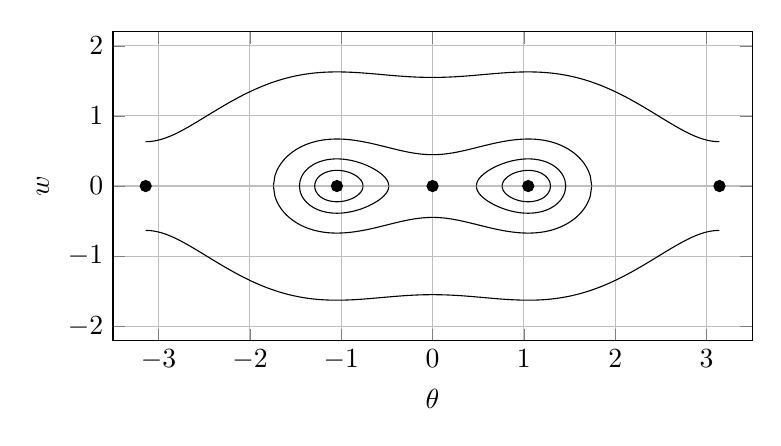
\begin{tikzpicture}
\begin{axis}[width=.8\textwidth,height=5.5cm,xlabel={$\theta$},ylabel={$w$},xmin=-3.5,xmax=3.5,ymin=-2.2,ymax=2.2,grid=major]
% Each plotted interval is physically allowed; max only suppresses endpoint rounding.
\foreach \en in {-.1,-.05}{
\pgfmathsetmacro{\lo}{acos((1+sqrt(1+8*\en))/2)*pi/180}
\pgfmathsetmacro{\hi}{acos((1-sqrt(1+8*\en))/2)*pi/180}
\foreach \sgn in {-1,1}{
\addplot[no marks,domain=\lo:\hi,samples=150]{\sgn*sqrt(max(0,2*(\en-.5*cos(deg(x))^2+.5*cos(deg(x)))))};
\addplot[no marks,domain=-\hi:-\lo,samples=150]{\sgn*sqrt(max(0,2*(\en-.5*cos(deg(x))^2+.5*cos(deg(x)))))};}
}
\pgfmathsetmacro{\turn}{acos((1-sqrt(1.8))/2)*pi/180}
\foreach \sgn in {-1,1}{
\addplot[no marks,domain=-\turn:\turn,samples=220]{\sgn*sqrt(max(0,2*(.1-.5*cos(deg(x))^2+.5*cos(deg(x)))))};
\addplot[no marks,domain=-pi:pi,samples=220]{\sgn*sqrt(2*(1.2-.5*cos(deg(x))^2+.5*cos(deg(x))))};}
\addplot[only marks,mark=*,mark size=2pt]coordinates{(0,0)(1.047197551,-0)(-1.047197551,0)(3.141592654,0)(-3.141592654,0)};
\end{axis}
\end{tikzpicture}

\begin{tikzpicture}
\begin{axis}[width=.8\textwidth,height=5.5cm,xlabel={$\theta$},ylabel={$w$},name=hoopMain,xmin=-1.7,xmax=6,ymin=-1.3,ymax=5.3,grid=major,legend pos=north east]
\addplot[no marks]table[x=theta,y=w,col sep=comma]{figures/hoop-0.csv};\addlegendentry{正斜点附近}
\addplot[dashed,no marks]table[x=theta,y=w,col sep=comma]{figures/hoop-1.csv};\addlegendentry{负斜点附近}
\addplot[dotted,no marks]table[x=theta,y=w,col sep=comma]{figures/hoop-2.csv};\addlegendentry{$(0,5)$出发}
\addplot[thin,dashed]coordinates{(3.141592654,-1.3)(3.141592654,5.3)};
\end{axis}
\begin{axis}[at={(hoopMain.south west)},anchor=south west,xshift=1.2cm,yshift=1.9cm,width=3.5cm,height=2.8cm,xmin=-.1,xmax=.2,ymin=-.12,ymax=.04,xlabel={$\theta-\pi/3$},ylabel={$w$},title={正平衡局部},axis background/.style={fill=white},ticklabel style={font=\scriptsize},label style={font=\scriptsize},title style={font=\scriptsize},xtick={0,.15},ytick={-.1,0}]
\addplot[no marks]table[x expr=\thisrow{theta}-pi/3,y=w,col sep=comma]{figures/hoop-0.csv};
\end{axis}
\begin{axis}[at={(hoopMain.south west)},anchor=south west,xshift=7.5cm,yshift=1.9cm,width=3.5cm,height=2.8cm,xmin=-.2,xmax=.1,ymin=-.04,ymax=.12,xlabel={$\theta+\pi/3$},ylabel={$w$},title={负平衡局部},axis background/.style={fill=white},ticklabel style={font=\scriptsize},label style={font=\scriptsize},title style={font=\scriptsize},xtick={-.15,0},ytick={0,.1}]
\addplot[no marks]table[x expr=\thisrow{theta}+pi/3,y=w,col sep=comma]{figures/hoop-1.csv};
\end{axis}
\end{tikzpicture}
\end{center}
上图是$b=0,\gamma=2$的有效能量等值线; 下图是$b=1,\gamma=2$的实际轨道, 竖虚线表示顶部$\theta=\pi$. 高初速轨迹确实越过此线, 随后耗散, 不能跨图混用守恒性.


\begin{exercise}
原题3（10分）. 无阻尼受迫摆$\dot\theta=w$, $\dot w=-\sin\theta-a\cos\phi$, $\dot\phi=\omega_D$, 取$\omega_D=.7$. (a) 至少300区间绘$.1<a<2$的截面参数图, 寻找混沌区域之间的周期窗口并以截面佐证. (b) 细查$0<a<.1$, 并测试$0<a<1$内最早出现混沌的位置.
\end{exercise}
\begin{solution}
按$T_D=2\pi/.7$采样, 相位初值$\phi(0)=0$, 本册固定$(\theta(0),w(0))=(.2,0)$. 无阻尼的二维变分流散度为零, 所以每周期Poincaré映射保面积. 因此原题参数图不能解释成“舍弃暂态后所有初值收敛到同一个吸引子”. 周期椭圆轨道周围常有不变曲线, 截面形成一圈点, 而不是阻尼模型中的单个吸引点.

本册用切向方程$\dot u=v$, $\dot v=-\cos\theta(t)u$估计有限时间增长率. 零阻尼下数值误差也会积累, 正的短时指数还可能只是临近分离轨道的暂态. 因此“最早混沌”必须注明起点、参数网格、观察长度与判据; 对全部初值作全局阈值声明需要额外理论.
宽区间和小区间都取301个参数值, 每周期384步, 先积分250周期, 再观察100周期. 宽扫描在$a=.252$首先达到本次人为选择的有限时间指数$.02$阈值, 而$0\le a\le.1$范围的最大估计约$.000489$, 本次观察未找到明确正增长证据. 阈值$.02$、网格间距、初值都是本次实验设置, $.252$不能称系统全局“最早混沌”精确值.

另外用自适应积分舍弃350周期后观察180周期, 复算$a=.2,.252,.05$的指数分别为$.000239,.09536,.000278$. $.2$和$.05$截面接近不变曲线, 在$1,2,4,8,16$次采样移位下均没有小回归误差, 不能将它们误标成有限周期. $.252$有稠密截面和持续正增长的数值证据. 小参数下未观察到混沌, 也不等于证明对全部初值无混沌.

按固定初值扫描未找到可认证的“吸引周期窗口”. 为检查周期结构, 本册另用射击法寻找相同驱动相位下的周期轨道并检验单周期变分矩阵, 结果见下一段. 局部周期岛与同参数其他初值的混沌可以共存, 所以不能把无阻尼模型压缩成一个与初值无关的窗口或第一混沌值.

射击法令相位0时$w(0)=0$, 对$\theta_0$求$w(T_D/2)=0$, 再用驱动的时间反射对称构成整周期轨道. $a=.3$时得到$\theta_0=-.6525804264$, 整周期闭合误差约$4.31\times10^{-11}$. 联立变分方程积分得单周期矩阵行列式$.9999999998$、迹$-1.1680801241$, 两本征值在单位圆上且非实, 是线性椭圆型周期轨道. 另从该点偏移$.002$作180周期采样, 得到围绕周期点的近闭截面曲线. 这给出局部周期轨道及邻近规则运动的数值证据, 与另一初值下的混沌可共存. 椭圆线性分类本身仍不能证明非线性全局稳定. 本题未给出一个对所有初值通用的周期吸引窗口或精确第一混沌参数, 读者复算时应保留此界限.

\end{solution}
\begin{center}
\foreach \name/\label/\xtspace in {pendulum-wide/{$.1\le a\le2$}/.5,pendulum-small/{$0\le a\le.1$}/.02}{
\begin{tikzpicture}
\begin{axis}[width=.85\textwidth,height=5cm,xlabel={$a$},ylabel={$\theta(nT_D)$},title={\label},xtick distance=\xtspace,scaled x ticks=false,xticklabel style={/pgf/number format/fixed,/pgf/number format/precision=2},ymin=-3.2,ymax=3.2]
\addplot[only marks,mark=square*,mark size=.13pt,black]table[x=a,y=theta,col sep=comma]{figures/\name-bifurcation-plot.csv};
\end{axis}
\end{tikzpicture}\par
}
\foreach \idx in {0,1,2}{
\begin{tikzpicture}
\begin{axis}[width=.72\textwidth,height=4.8cm,xlabel={$\theta\pmod{2\pi}$},ylabel={$w$},title={独立复算案例 \idx},xmin=-3.2,xmax=3.2]
\addplot[only marks,mark=*,mark size=.6pt]table[x=theta,y=w,col sep=comma]{figures/pendulum-section-\idx.csv};
\end{axis}
\end{tikzpicture}\par
}
\begin{tikzpicture}
\begin{axis}[width=.44\textwidth,height=4.8cm,xlabel={$\theta$},ylabel={$w$},title={$a=.3$周期轨道}]
\addplot[no marks]table[x=theta,y=w,col sep=comma]{figures/pendulum-periodic-orbit.csv};
\end{axis}
\end{tikzpicture}\hfill
\begin{tikzpicture}
\begin{axis}[width=.44\textwidth,height=4.8cm,xlabel={$\theta-\theta_0$},ylabel={$w$},title={周期点邻近截面},scaled x ticks=false,xticklabel style={/pgf/number format/fixed,/pgf/number format/precision=3}]
\addplot[only marks,mark=*,mark size=.55pt]table[x=theta_offset,y=w,col sep=comma]{figures/pendulum-periodic-island-offset.csv};
\end{axis}
\end{tikzpicture}
\end{center}
截面将角度折回$[-\pi,\pi)$; 图边两侧点可能属于同一圆柱相空间轨道, 不能把折回产生的跳跃误当不连续动力学. 参数与有限时间诊断在题下及数值报告中逐项给出.


\begin{exercise}
原题4（12分）. $\ddot x+a\dot x(x^2+\dot x^2-1)+x=0$. (a) 写一阶系统, 证明$a\ne0$时有圆形极限环, 给振幅和周期. (b) 分类$a>0,a<0,a=0$的固定点, 提出环稳定性判断. (c) 转极坐标推导$\dot r$并证明判断, 给分岔点与合理名称.
\end{exercise}
\begin{solution}
令$w=\dot x$, 方程$\dot x=w$, $\dot w=-x-aw(x^2+w^2-1)$. 仅有固定点$(0,0)$, 线性根$\lambda_\pm=(a\pm\sqrt{a^2-4})/2$. $a>0$不稳定, $0<a<2$焦点、$a>2$结点; $a<0$稳定, $-2<a<0$焦点、$a<-2$结点. $a=\pm2$重根, $a=0$为线性中心. 原题不要求深入重根边界分类.

取$x=r\cos\vartheta,w=r\sin\vartheta$, 直接以$(x\dot x+w\dot w)/r$和$(x\dot w-w\dot x)/r^2$计算得
\[
\dot r=-ar\sin^2\vartheta(r^2-1),\qquad
\dot\vartheta=-1-a\sin\vartheta\cos\vartheta(r^2-1).
\]
$r=1$时$\dot\vartheta=-1$, 故精确圆解$x=\cos(t+\delta),w=-\sin(t+\delta)$, 振幅1、周期$2\pi$. $a>0$时$0<r<1$径向不减、$r>1$不增. 除$w=0$的瞬时点外符号严格; 轨道不能一直滞留$w=0$（该线上$\dot w=-x$）, 因而原点之外的轨道趋向$r=1$. 形式上可用$E=r^2/2$的单调性及最大不变集论证. $a<0$箭头全部反向, 圆环双侧排斥, 原点吸引其内侧轨道. 这也证明$a\ne0$时不存在邻近的其他周期圆, 环是孤立的.

$a=0$所有$r$常数, 全部非零圆都是周期轨道而不孤立, 原点为中心. 分岔点$a=0$, 圆环与原点交换稳定性; 由于环半径始终1, 它不是通常小振幅随参数连续生出的非退化Hopf分岔. 可称退化的中心--焦点/极限环稳定性交换分岔, 需说明此名称所指的具体行为.
\end{solution}

\begin{exercise}
原题5（15分）. Logistic映射$x_{n+1}=rx_n(1-x_n)$. (a) 选周期、混沌参数各一, 画两近初值之差, 求确保$|x_{15}-x'_{15}|<10^{-6}$的初差条件. (b) 找前四个倍周期参数$a_1,\ldots,a_4$, 算两相邻间距比. 原件此处称“x values”, 实际横轴控制量为$r$, 本册按其意图解释. (c) 证明一、二次分岔间的二周期点满足$r^3x^2(2-x)-r^2(r+1)x+(r^2-1)=0$. (d) 为$r\cos x$、$rx-x^3$、$e^{-rx}$三映射画包含倍周期的参数图, 对能混沌的两例包含有序/混沌区域.
\end{exercise}
\begin{solution}
(a) 取$r=3.2$与4, 初值$.2$和$.2+10^{-10}$, 实际差值见下图. 周期情形差值渐消（最终受浮点舍入影响）; $r=4$初差在典型轨道上放大并达到宏观量级. 若两初值都在$[0,1]$, $|f'(x)|\le4$, 逐次均值定理给$|x_{15}-x'_{15}|\le4^{15}|x_0-x'_0|$. 因此$|x_0-x'_0|<10^{-6}/4^{15}\simeq9.3132\times10^{-16}$是对所有此域初值成立的充分条件, 不是必要条件. 特定轨道可用15步导数乘积给更宽条件; 典型Lyapunov指数估计$\ln2$不能代替保证. 浮点双精度在这量级需留舍入裕度, 严格保证应使用高精度或误差包络.

(b) 周期$p$的倍周期边界可同时求$f^p(x)-x=0$和$\prod_{k=0}^{p-1}f'(x_k)=-1$, 不必靠手读粗图. 本册从实际数值根求得
\[
\begin{aligned}
a_1&=3, & a_2&=3.4494897428,\\
a_3&=3.5440903596, &a_4&=3.5644072661.
\end{aligned}
\]
相邻比$(a_2-a_1)/(a_3-a_2)=4.7514462$, $(a_3-a_2)/(a_4-a_3)=4.6562510$, 两者相差约2\%, 按两位有效数字分别为4.8与4.7, 不应声称已经完全一致. 原题希望观察相邻比趋近同一常数, 前两阶只给有限阶近似; 要提高一致程度需继续求更高阶, 也未由四点证明极限普适常数.

(c) 令$f(x)=rx(1-x)$, 直接展开并对非零$x$除去因子$x$, $f(f(x))-x=0$化成题中三次式. 它同时含非零固定点$(r-1)/r$, 因而满足该式本身不足以证明最小周期2. 再除固定点因子得到$r^2x^2-r(r+1)x+(r+1)=0$, 两根$x_\pm=(r+1\pm\sqrt{(r-3)(r+1)})/(2r)$. 在$3<r<1+\sqrt6$二周期乘子$-r^2+2r+4$绝对值小于1, 所以是稳定吸引二周期.

(d) 下面图取固定$x_0=.2$, 舍弃2000次, 再画40次; 余弦取$0\le r\le3$, 三次映射取$1\le r\le2.59$, 指数映射取$0\le r\le10$. 三次映射在更大参数会逃逸, 不该把溢出的数值点解释成混沌吸引子. 指数映射严格递减, 其二次迭代递增; 有界轨道只能趋向固定点或二周期, 不会沿无限倍周期链混沌. 在固定点$x_*=e^{-rx_*}$, 导数为$-rx_*$, 首次翻转阈值$rx_*=1$给$r=e$, 与图一致. 前两例图示倍周期和更复杂非周期点集, 数值图仍不替代严格混沌证明.
\end{solution}
\begin{center}
\begin{tikzpicture}
\begin{axis}[width=.85\textwidth,height=5.2cm,xlabel={$r$},ylabel={$x_n$},xmin=3,xmax=4,ymin=0,ymax=1]
\addplot[only marks,mark=square*,mark size=.12pt,black]table[x=r,y=x,col sep=comma]{figures/logistic-bifurcation-plot.csv};
\end{axis}
\end{tikzpicture}

\begin{tikzpicture}
\begin{semilogyaxis}[width=.85\textwidth,height=5cm,xlabel={$n$},ylabel={$|x_n-x'_n|$},legend pos=north west,ymin=1e-17,ymax=1,grid=major]
\addplot[no marks]table[x=n,y=delta,col sep=comma]{figures/map-sensitivity-periodic.csv};\addlegendentry{$r=3.2$}
\addplot[dashed,no marks]table[x=n,y=delta,col sep=comma]{figures/map-sensitivity-chaotic.csv};\addlegendentry{$r=4$}
\end{semilogyaxis}
\end{tikzpicture}

\foreach \name/\label in {cosine/$r\cos x$,cubic/$rx-x^3$,exponential/$e^{-rx}$}{
\begin{tikzpicture}
\begin{axis}[width=.85\textwidth,height=5cm,xlabel={$r$},ylabel={$x_n$},title={\label}]
\addplot[only marks,mark=square*,mark size=.12pt,black]table[x=r,y=x,col sep=comma]{figures/\name-map-plot.csv};
\end{axis}
\end{tikzpicture}\par
}
\end{center}
上面散点来自实际迭代, 绘图为清晰起见抽稀点集; 参数扫描与原始数据保留在源码. 指数映射只出现固定点和二周期, 与严格单调性的分析一致.

